%%%%%%%%%%%%%%%%%%%%%%%%%%%%%%%%%%%%%%%%%
% Beamer Presentation
% LaTeX Template

\documentclass{beamer}
\mode<presentation> {
% Theme
\usetheme{metropolis}
%\usetheme[background=dark]{metropolis}
%\setbeamertemplate{footline} % To remove the footer line in all slides uncomment this line
%\setbeamertemplate{footline}[page number] % To replace the footer line in all slides with a simple slide count uncomment this line
%\setbeamertemplate{navigation symbols}{} % To remove the navigation symbols from the bottom of all slides uncomment this line
}

%Packages
\usepackage{graphicx} % Allows including images
\usepackage{booktabs} % Allows the use of \toprule, \midrule and \bottomrule in tables
%\usepackage{cite}
\usepackage[numbers]{natbib} % For bibliography
\usepackage{multirow}
\usepackage{hyperref}
%\usetheme{Warsaw}
\usepackage[absolute,overlay]{textpos}


% Prepare title and TOC
\title[Short title]{Reproducible Research -- practical} 
\author{Marco Chiapello} 
\institute[Center for Proteomics] 
{
Center for Proteomics\\
University of Cambridge \\ 
\medskip
\textit{mc983@cam.ac.uk} 
}
\date{\today} 

%\AtBeginSectfon[]
%{
%\begin{frame}<beamer>
%\frametitle{Overview}
%\tableofcontents[currentsection]
%\end{frame}
%}


%-------------------------------------------
% MAIN DOCUMENT
%-------------------------------------------
\begin{document}

%-------------------------------------------
% TITLE PAGE
%-------------------------------------------
\begin{frame}
\titlepage 
\end{frame}

%----------------------------------------------------------------------------------------
%	PRESENTATION SLIDES
%----------------------------------------------------------------------------------------
\begin{frame}
    \section{RMarkdown}
    
\includegraphics[scale=0.45]{figures/RMarkdownFlow.png}
\end{frame}
%---------------
\begin{frame}
    \frametitle{Markdown}
    \Large{\bf Markdown} is a simple \underline{formatting language} designed to make authoring content easy for everyone. Rather than write in complex markup code (e.g. HTML or LaTex), you \underline{write in plain text} 
\end{frame}
%-----------
\begin{frame}
    \frametitle{Markdown}
    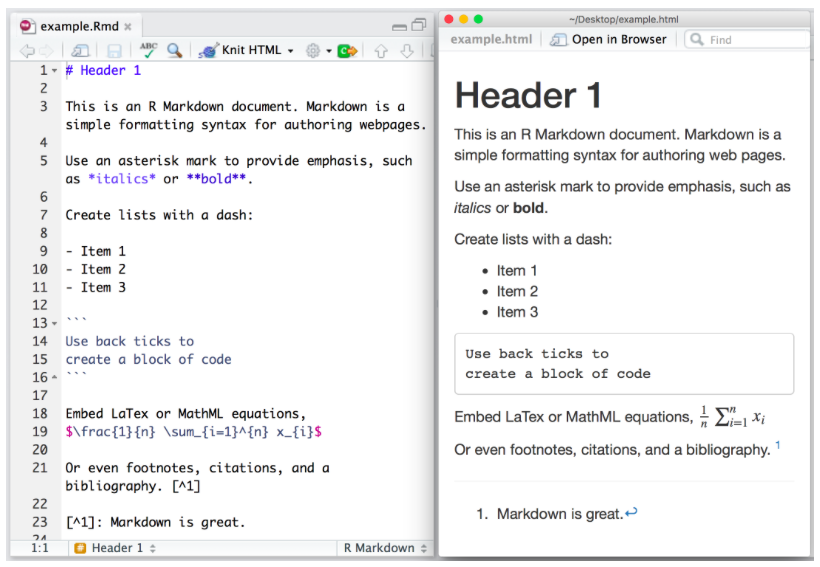
\includegraphics[scale=0.4]{figures/RmarkdownExample1.png}
\end{frame}
%----------
%------------------------
% Element explanation
%------------------------
\begin{frame}
    \frametitle{RMarkdown elements}
    \begin{itemize}
        \item Header
        \item Text
	\item Inline \texttt{R} code
        \item Code chunks
    \end{itemize}
\end{frame}

%-----------------
\begin{frame}
    \frametitle{RMarkdown elements}
    \centering \Large Header
    \normalsize
    	\begin{itemize}
		\item R Markdown documents can contain a metadata section that includes title, author, and date information 
		\item As well as options for customizing output
	\end{itemize}
	\begin{center}	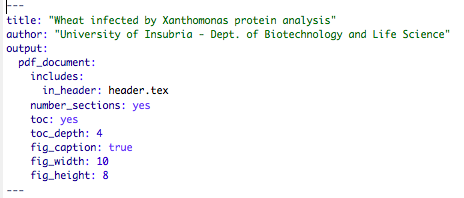
\includegraphics[scale=0.6]{figures/RMarkdown_hearder.png} \end{center}
    
\end{frame}

\begin{frame}
    \frametitle{RMarkdown elements}
    \centering \Large Text
    \normalsize
    	\begin{itemize}
		\item Text can be added to comment you code
		\item Text can be added to comment your outputs
	\end{itemize}
	\begin{center}	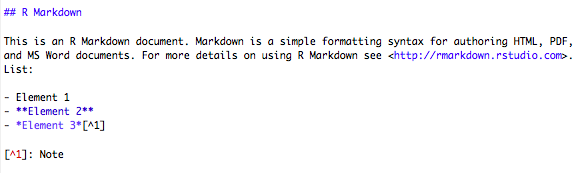
\includegraphics[scale=0.6]{figures/RMarkdown_text.png} \end{center}
\end{frame}

\begin{frame}
    \frametitle{RMarkdown elements}
	\centering \Large Inline \texttt{R} code
	\normalsize
	\begin{itemize}
		\item \texttt{R} expressions can be evaluated inline 
		\item Enclosing the expression within a single back-tick qualified with ‘r’.
	\end{itemize}
	\begin{center}	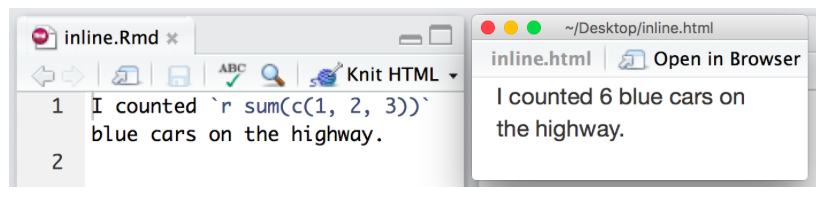
\includegraphics[scale=0.4]{figures/RMarkdown_inline.png} \end{center}
\end{frame}

%-----------
\begin{frame}
    \frametitle{RMarkdown elements}
	    \centering \Large \texttt{R} chunck
	\begin{itemize}
		\normalsize
		\item \texttt{R} Code Chunks can be embedded with the native Markdown syntax for fenced code regions
	\end{itemize}
    \begin{center}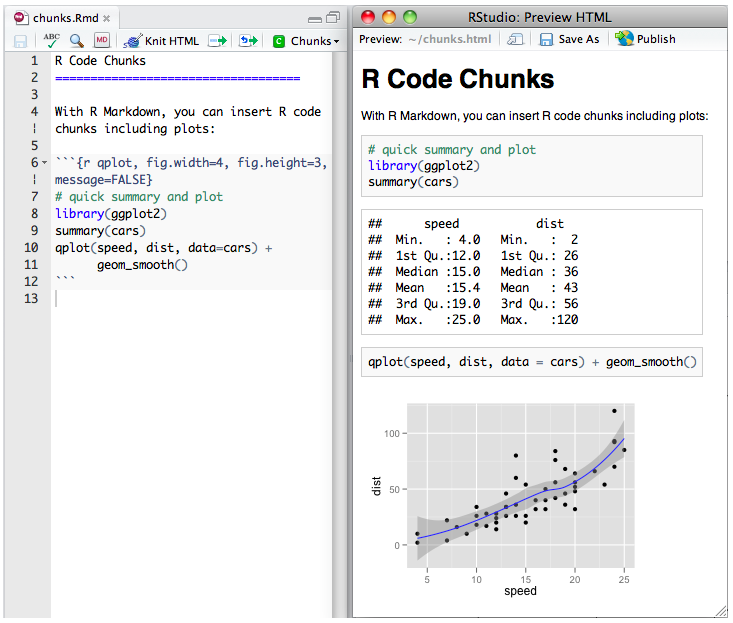
\includegraphics[scale=0.35]{figures/RmarkdownExample2.png}\end{center}
\end{frame}


\begin{frame}
    \frametitle{RMarkdown elements}
	    \centering \Large \texttt{R} chunck options \tiny[few of them]

	    \normalsize There are six types of output:
	\begin{itemize}
		\normalsize
		\item \textbf{source code}: use chunk option \underline{'echo'}, e.g. echo=FALSE hides the R code
	\pause
		\item \textbf{normal text output}: use option results (\underline{'markup'} marks up the results; \underline{'asis'} return texts as-is; \underline{'hide'} hides the results)
	\pause
		\item \textbf{messages}: option message (\underline{'FALSE'} hides messages in the output)
	\pause
		\item \textbf{warnings}: option warning (\underline{'FALSE'} hides warnings in the output)
	\pause
		\item \textbf{errors}: option error (\underline{'FALSE'} will make R stop if an error occurs; \underline{'TRUE'} will show the error messages in the output)
	\pause
\item \textbf{plots}: option \underline{'fig.keep'} (\underline{'none'} discards all plots; \underline{'all'} for all plots including low-level plots; \underline{'high'} for high-level plots)
	\end{itemize}
\end{frame}





%-----------
% Exercise 1 
%-----------
\begin{frame}
    \frametitle{Exercise 1}
    {\sc GOAL: create a default minimal document}
    \begin{itemize}
        \item Open RStudio
            \pause
        \item Select File $>$ New file $>$ R Markdown
            \pause
        \item Create an HTML document
    \end{itemize}
\end{frame}
%-----------------------
\begin{frame}
    \frametitle{Exercise 1}
    \begin{center}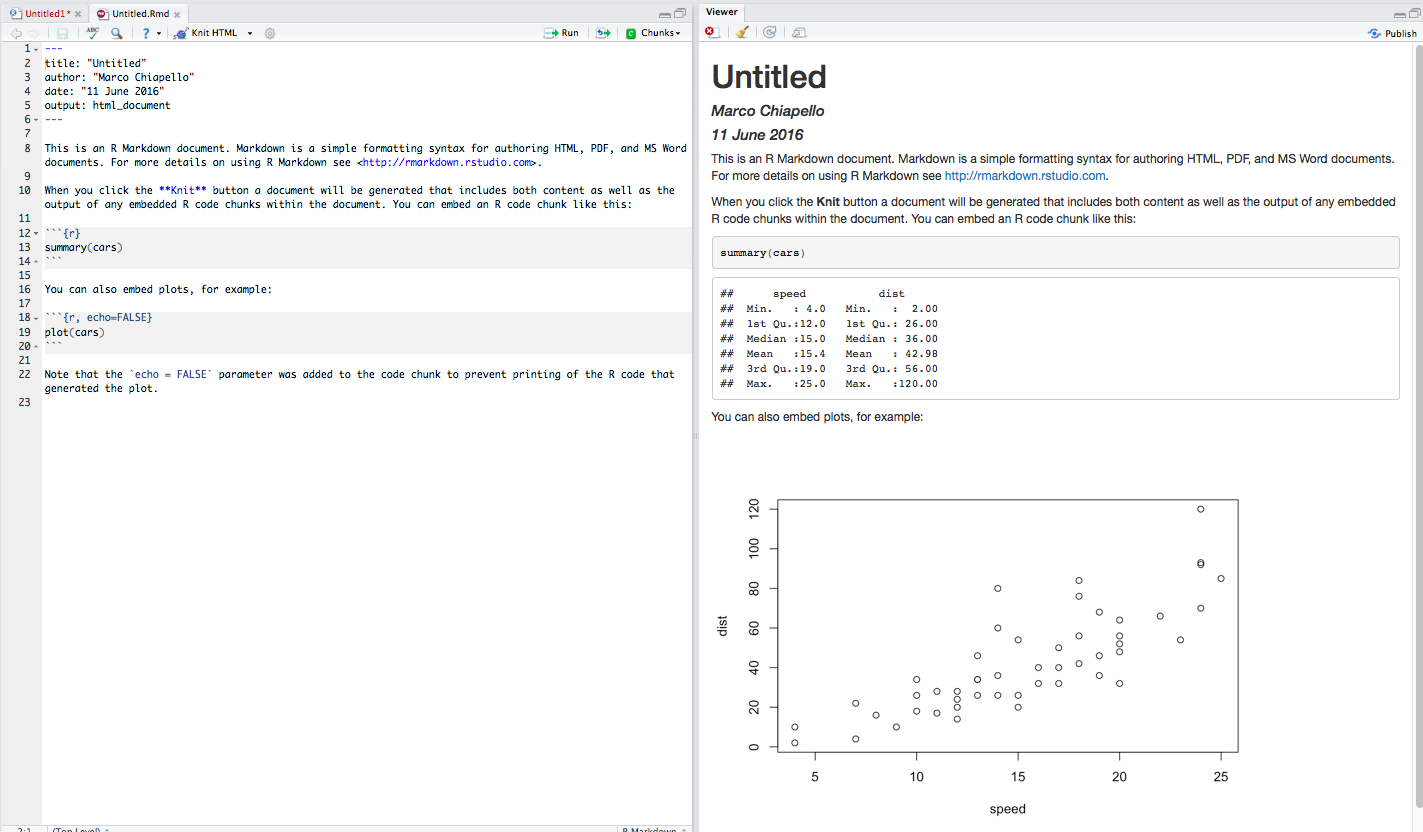
\includegraphics[scale=0.23]{figures/RmarkdownExample.png}\end{center}
\end{frame}
%-----------------------
\begin{frame}
    \frametitle{Exercise 1}
    {\sc GOAL: create a default minimal document}
    \begin{itemize}
        \item Open RStudio
        \item Select File $>$ New file $>$ R Markdown
        \item Create an HTML document
	\item Suppress the printing of the \texttt{R} code
		\pause
	\item Suppress the printing of the \texttt{R} results
		\pause
	\item Suppress the printing of the plot
    \end{itemize}
\end{frame}
%-----------------------

%-------------
% Exercise 2
%-------------
\begin{frame}
    \frametitle{Exercise 2}
    {\sc GOAL: create a default minimal document in other formats}
    \begin{itemize}
        \item Create a pdf document
        \item Create a docx document
    \end{itemize}
\end{frame}

%-------------
% Exercise 3
%-------------
\begin{frame}
    \frametitle{Exercise 3}
    {\sc GOAL: create a RMarkdown document}
    \begin{itemize}
        \item Using the dataset4.csv
        \item Create a document containing analysis, plots and comments
	\pause
	\item Run your Rmarkdown document using 'dataset5.csv'
    \end{itemize}
\end{frame}


\end{document}

